\documentclass{llncs}

\usepackage[T1]{fontenc}
\usepackage[utf8]{inputenc}
\usepackage{url}
\usepackage{graphicx,times,amsmath}
\usepackage{multirow}
\usepackage{listings}
\usepackage{float}

\usepackage{hyperref}
\hypersetup{
 bookmarks=true, 
 bookmarksopen=true, %les afficher complètement.
 pdftitle={ReqHunter - a Requirements Management Tool}, %informations apparaissant dans
 pdfauthor={Nicolas James}, %dans les informations du document 
 pdfsubject={} %sous Acrobat.
}

\title{ReqHunter - a Requirements Management Tool}

\author{Nicolas James}

\institute{Space Applications Services\\
nicolas.james@spaceapplications.com}

\begin{document}

\maketitle

\section{General context}
In the framework of the RARE project\footnote{http://rssportal.esa.int/deepenandlearn/tiki-index.php?page=RARE+Project} at Space Applications Services, we had the need of a requirement management tool. After a review of the available tools, it seems that it is still difficult to find a software or a set of tools that is: (1) not necessarily user friendly but simple to use, (2) easy to install, (3) extendable to our business logic, and (4) that produces outputs as it was required in the RARE project.

Furthermore few other points lead us to work on this new tool. 

First is that we have discovered only few tools that allow to extract content from a Word document to constitute an initial version of a requirements database. This feature, i.e. to extract content from a Word document, is an important one because it is often the case that the first draft issued from a requirements listing process is written in a Microsoft Word document. Why this type of file? There are several reasons but the main is the multiple inputs: some inputs are coming from partners, others inputs are extracted from user questionnaires etc. In order to constitute a list of requirements, a Word document is hence the best choice since the requirements are the result a \textit{patchwork} of documents and information. To be able to extract content from Word document is valuable and allow to constitute an initial version of a requirements database. 

However extracting content from a Word document is not an easy task, firstly because of the Word .doc format (although it is easier with the .docx format), secondly the conception of a graphical user interface for enabling the user to specify the content to extract is not an easy task. In ReqHunter, you have to write Java code to extract content from a Word document (using Apache POI), but all the needed environment is available to do it properly.

The second point that leads us to work on ReqHunter is that the task of managing requirements may be improved by semantic and semantic web technologies. We have not seen such an approach in the review of the available requirements management software. The software do not include such semantic features for now. This is an open perspective and the project is a good candidate to develop it.

\section{Review of the available software}

\subsection{XStudio}
XStudio, http://www.xqual.com/products/xstudio.html
It seems that there is no generation of reports available (Word documents, listing of the requirements etc.).
The software is GPL?
Requirements, Specifications, Tests.
There is Tests campaigns, which is very interesting...
It seems strongly related to test tools and software.
Generation in HTML and XML.
Import/export in CSV and XML.

\subsection{RequisitePro}

IBM Rationale RequisitePro, http://www-01.ibm.com/software/awdtools/reqpro/

\subsection{Doors}

IBM Rationale Doors, http://www-01.ibm.com/software/awdtools/doors/

\subsection{CaliberRM}

Borland Caliber Requirement Management, http://www.borland.com/us/products/caliber/

\subsection{ReqLine}

http://pragnalysis.com/index.php?option=com\_content\&view=article\&id=111

MS-Windows only, developed using .Net.

The ReqLine application is a totally free .Net application that allows you to manage requirements and other important project information in a central repository. The tool is a single user application designed to sit between using MS Office to manage requirements, via spreadsheets or Word documents, and the large commercial multiuser applications that operate at an Enterprise level. This software is not a client/server software. 

\subsection{UNICASE}

http://code.google.com/p/unicase/

UNICASE is a SWT\footnote{http://www.eclipse.org/swt/} application and a plugin for the Eclipse Integrated Development Environment. UNICASE is a CASE-tool (a Computer-Aided Software Engineering tool) that supports modeling artifacts of a software engineering project. The software use a database but can be a local database or a distant database. 

\subsection{TopCased}

http://www.topcased.org/index.php

TopCased is an Eclipse plugin, and since recently works with Papyrus which is an environment for editing any kind of EMF model and particularly supporting UML and related modeling languages such as SysML and MARTE. Papyrus provides diagram editors for EMF-based modeling languages amongst them UML 2 and SysML and the glue required for integrating these editors (GMF-based or not) with other MBD and MDSD tools.

\subsection{RMTrack}

https://www.rmtrak.com/home.aspx

There is no free version of RMTrack available.

\subsection{rmtoo}

http://www.flonatel.de/projekte/rmtoo/

RMTOO is a very promising tool for managing requirements. It is a young project but several valuable features are already implemented.
There is no traceability matrix. The output of the project use Latex.
A valuable feature is the generation of a depency graph of the requirement.
Each requirement is specified in a file with the extension .req. The format of the requirements is internal to rmtoo, and this is the most important critique we can do to rmtoo.
Unfortunately, the software is develop using the KISS (Keep It Simple Stupid) principle and the tool is maybe a bit difficult to use, furthermore if we want to implement a RefenceFactory for give to each requirement a unique reference (in the scope of a project).

\subsection{OSRMT}

This project is dead. However there is a successor http://sourceforge.net/projects/nimble.

It is a full web application.

\subsection{REMA}

Requirement Manager, REMA, http://www.rema-soft.com/index.html

Seems very promising, to investigate.

\subsection{Conclusion}

\section{ReqHunter}

ReqHunter is not user friendly. To use this software you need to implement the ReqHunter API. This API is very simple and straighforward, but as this implementation is required we can say that users of ReqHunter are mostly Java developers or people that know a bit of Java programming. It is a constraint in the usage of the software but hence you can define the structure of your requirements, the format of the references (associated to each requirement) and a lot of things.\\
\\
The real interest of Reqhunter is to provide a environment for working on the user requirements easily.
\\
Examples of requirements are given Table \ref{table:rmtoo_req} which contains a requirement from rmtoo and Table \ref{table:rare_req} which contains a requirement from the RARE project.

\begin{figure}[H]
	\centering
	\begin{tabular}{ | p{\linewidth} | }
	\hline
	\textbf{Name:} Analytics \\
	\textbf{Type:} requirement \\
	\textbf{Invented on:} 2010-08-05 \\
	\textbf{Invented by:} flonatel \\
	\textbf{Description:} The requirements \textbf{must} be analyzed. \\
	\textbf{Rationale:} It is hard to write good requirements - as far as possible rmtoo should support writing good requirements. \\
	\textbf{Note:} Analytics are implemented using modules with a defined interface. \\
	\textbf{Owner:} development \\
	\textbf{Status:} finished \\
	\textbf{Priority:} development:10 \\
	\textbf{Effort estimation:} 5 \\
	\textbf{Topic:} Basics \\
	\textbf{Solved by:} AtcsDescWords AtcsHotSpot AtcsReqTopicCohe AtcsTopicCohe \\
	\hline
	\end{tabular}
	\caption{A requirement from rmtoo}
	\label{table:rmtoo_req}
\end{figure}

\begin{figure}[H]
	\centering
	\begin{tabular}{ | p{\linewidth} | }
	\hline
	\textbf{Id:} UR-AI-040 \\
	\textbf{Category:} UR-AI \\
	\textbf{Name:} The RARE software shall include an administration interface. \\
	\textbf{Priority:} M \\
	\textbf{Description:} This administration interface shall include: management of the RRS ontology, the RRS knowledge base and management of the modules and services. \\
	\textbf{Verification:} T \\
	\textbf{Source:} SoW I8.7.* \\
	\hline
	\end{tabular}
	\caption{A requirement from the RARE project}
	\label{table:rare_req}
\end{figure}

These two type of requirements are very different. First their structures are different, the number of fields and their names. The semantics attached to each field is different. And constraints underlying the values of some fields (as the field "Effort estimation" in Table \ref{table:rmtoo_req} or the field "Priority" in Table \ref{table:rare_req}) may exists.

ReqHunter is composed of three processes:
\begin{enumerate}
  \item context extraction,
  \item requirement management,
  \item applicable document generation.
\end{enumerate}

Figure \ref{fig:reqhunter_api} represents the UML class diagram the three classes to implement.

\begin{figure}[H]
	\centering
	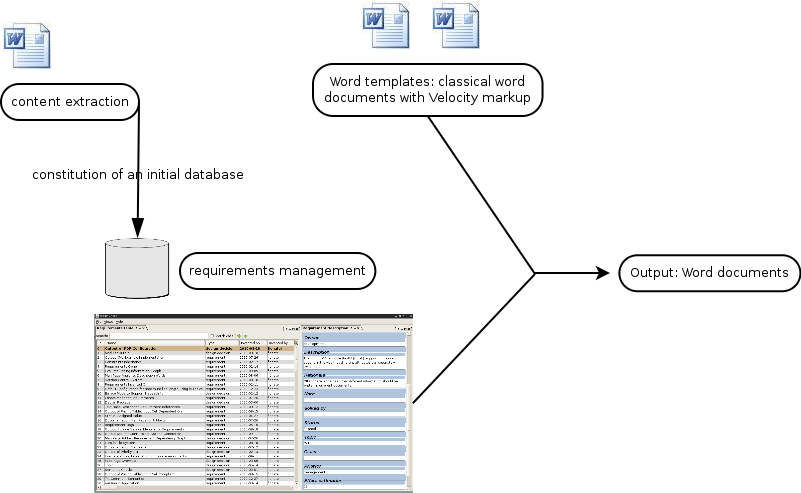
\includegraphics[width=\linewidth]{Diagram1.png}
	\caption{ReqHunter}
	\label{fig:reqhunter}
\end{figure}

To use ReqHunter you need at least two things: (1) a XML schema that represents your requirements, and (2) an implementation of the three classes in Figure \ref{fig:reqhunter}.

\begin{figure}[H]
	\centering
	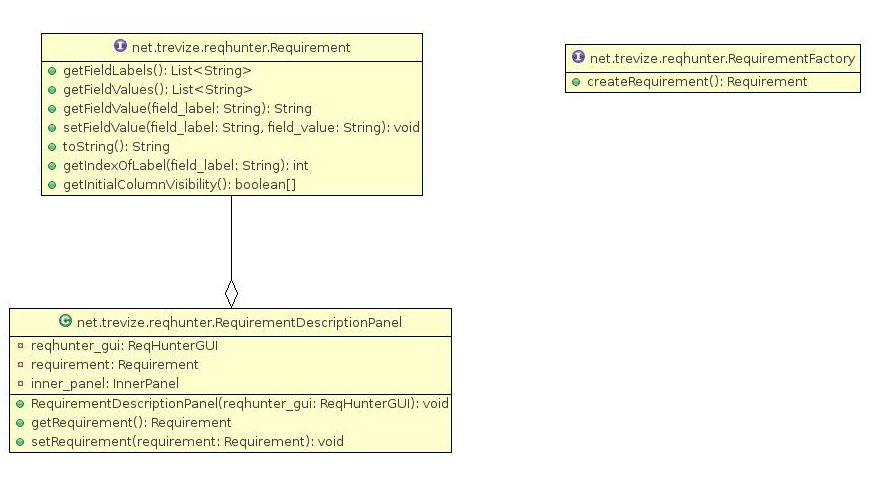
\includegraphics[width=\linewidth]{ReqHunter_API-1.jpg}
	\caption{UML class diagram of the ReqHunter API}
	\label{fig:reqhunter_api}
\end{figure}

\subsection{Writing a XML schema for your type of requirement}

Figure \ref{table:schema_req} is a example of a schema for the requirement type defined for the RARE project.

\begin{figure}[H]
	\centering
	\begin{tabular}{ | p{\linewidth} | }
	\hline
	\lstinputlisting[language=xml,tabsize=2,breaklines=true]{./RARE-requirement.xsd} \\
	\hline
	\end{tabular}
	\caption{The schema for the RARE requirements}
	\label{table:schema_req}
\end{figure}

\subsection{Implementation of the API}

The ReqHunter API is very short and simple:
\begin{itemize}
  \item net.trevize.reqhunter.Requirement: this class is an extension of the RequirementT class that JAXB produces from your XML Schema.
  \item net.trevize.reqhunter.RequirementFactory: this class is used by JAXB, you have to specify to JAXB that your implementation of this class is the factory of your type of requirement.
\end{itemize}

Using these two classes, ReqHunter is able to create, load and store requirements.

\subsection{Content extraction}

The content extraction process is provided by the Apache POI library (the Java API for Microsoft Documents), http://poi.apache.org/.

\begin{itemize}
  \item The extraction is fairly based on the style associated to paragraphs. You have to define a specific style for the content you want to extract.
  \item Execute the code located in net.trevize.rare.WordDocExtractor to list the styles encapsulated in your Word document.
  \item Search for the styles you have defined and modify the class net.trevize.rare.WordDocExtractor to parse your content and create Requirement objects (actually your implementation of the Requirement interface).
\end{itemize}

\begin{figure}[H]
	\centering
	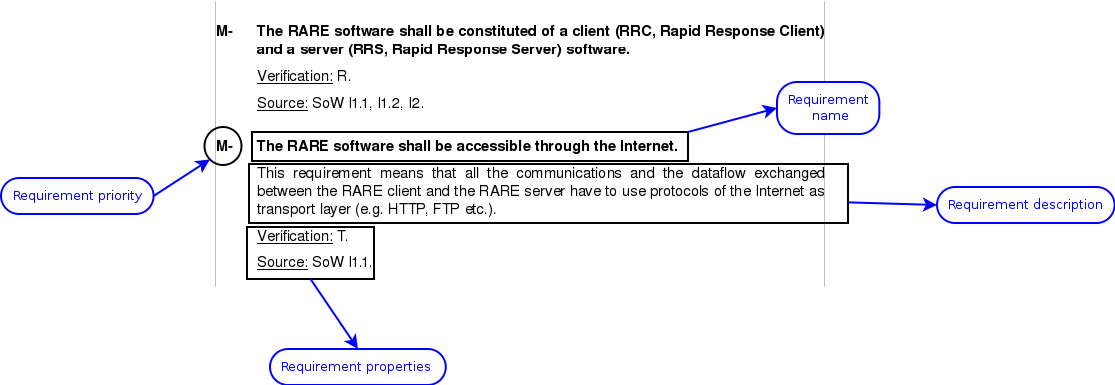
\includegraphics[width=\linewidth]{import_req_illu.png}
	\caption{Screenshot of a Word document and a user requirement.}
	\label{fig:import_illu}
\end{figure}

\subsection{Requirements database}

Use net.trevize.reqhunter.ReqHunter to refine your initial requirement database (if you have not skip the "Content extraction" step), or populate your empty requirement database.

Add screenshots, help about the interface etc.

\subsection{Applicable documents production}

To produce Word document from the requirement database, first create a new Word Document and follow the instruction here http://code.google.com/p/xdocreport/wiki/DocxReportingJavaMainListField

It could be a listing of the requirements, a traceability matrix etc.

\end{document}
